\subsection{Introduction to Quadcopter Systems}

A drone, also known as an unmanned aerial vehicle (UAV), is an aircraft without a human pilot \parencite{kangunde_review_2021}. Among different types of drones, a quadcopter, also frequently referred to as a quadrotor, is a type of multirotor helicopter or rotary-wing UAV that utilizes four rotors to achieve flight \parencite{luukkonen_modelling_2011}. These rotors are typically directed upwards and arranged in a square formation, with each rotor positioned at an equal distance from the center of mass. In this configuration, the four actuators are generally equally spaced by 90° from one another \parencite{idrissi_review_2022}.

The origins of quadrotor technology date back to 1907, when the Breguet brothers constructed the Gyroplane No. 1. While this marked one of the first manned helicopter flights, it was not a free flight; the machine lacked inherent stability and a proper control mechanism, requiring it to be tethered to the ground \parencite{ghazbi_quadrotors_2016}.

The transition to modern UAVs occurred in the late 1990s. A pivotal moment was the 1999 release of the Draganflyer I, the first camera-equipped quadrotor to achieve mass production. This shifted quadrotor technology from a laboratory curiosity to a viable commercial product \parencite{karahan2025development}.

Since 2010, advancements in micro-electronics and control theory have expanded the use of quadrotors across various sectors:

\begin{itemize}
    \item Public Safety: Search and rescue, firefighting, and border surveillance.
    \item Agriculture: Precision seeding, chemical spraying, and crop monitoring.
    \item Commercial: Last-mile delivery and high-end cinematography.
\end{itemize}


\subsubsection{Flight Dynamics and Principles of Operation}

A quadcopter is a common subcategory and represents an under-actuated system. As shown in \cref{fig:body}, it must manage six degrees of freedom (6DOF)—three translational and three rotational—using only four control inputs, namely the angular velocities of its rotors.

\begin{figure}
    \caption{The inertial and body frames of a quadcopter}\label{fig:body}
    \centering
    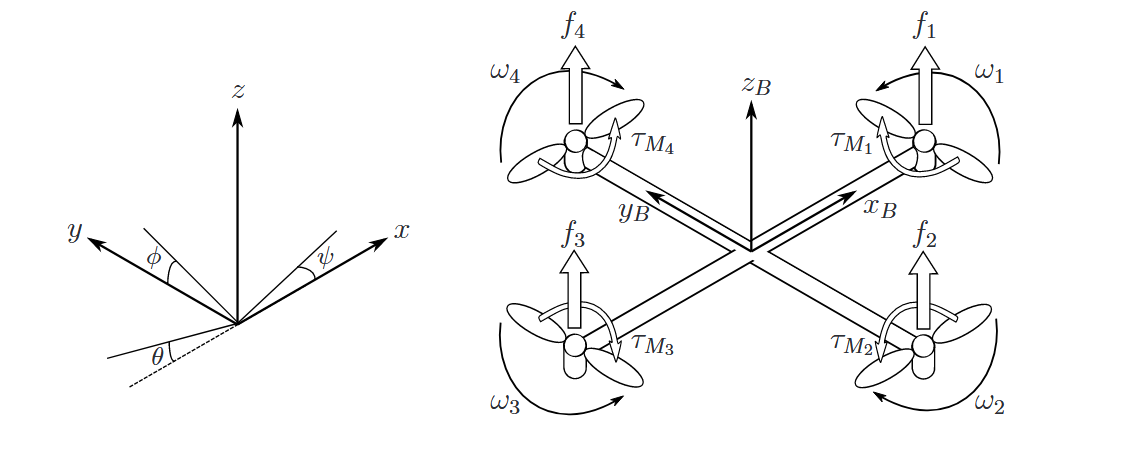
\includegraphics[width=0.8\linewidth]{img/6DOF.png}
\end{figure}

The fundamental principle of quadcopter stability relies on torque cancellation. To maintain a stable orientation, two motors rotate clockwise (CW) while the adjacent pair rotates counter-clockwise (CCW). This arrangement ensures that the net moment about the center of mass is zero; without this pair-wise opposition, the drone would rotate uncontrollably around its vertical axis. Quadcopters typically use either a plus (+) or cross (x) configuration, with the cross configuration being more common due to its superior stability \parencite{idrissi_review_2022}.

The absolute linear position of the quadcopter is defined in the inertial frame axes (${[x,y,z]}^T$). The attitude, i.e. the angular position, is defined in the inertial frame with three Euler angles (${[\phi, \theta, \psi]}^T$), which represent pitch angle, roll angle and yaw angle as shown in \cref{fig:body}.

Every change in position or attitude is achieved by varying the individual angular velocities ($\omega_i$) of the four rotors:

Thrust ($T$): Simultaneously increasing all rotor speeds causes the vehicle to ascend. The force generated by rotor $i$ is $f_i = k\omega_i^2$, where $k$ is the lift constant. Total thrust is defined as show in \cref{eq:T}

\begin{equation}\label{eq:T}
    T = k\sum_{i=1}^4\omega_i^2
\end{equation}

Yaw ($\tau_\psi$): Rotating the drone around the vertical axis is achieved by creating a torque imbalance between the CW and CCW pairs shown in \cref{eq:Y}, where $b$ is the drag constant.

\begin{equation}\label{eq:Y}
    \tau_\psi = b (\omega_1^2 - \omega_2^2 + \omega_3^2 - \omega_4^2)
\end{equation}

Roll ($\tau_\phi$) and Pitch ($\tau_\theta$): These are achieved by creating a speed differential between opposite rotors. For a distance $l$ from the center of mass, shown in \cref{eq:RP}

\begin{equation}\label{eq:RP}
\begin{gathered}
    \tau_\phi = l k (-\omega_2^2 + \omega_4^2) \\
    \tau_\theta = l k (-\omega_1^2 + \omega_3^2)
\end{gathered}
\end{equation}

The quadcopter is modeled as a rigid body using Newton-Euler equations. The acceleration in the inertial frame ${[x,y,z]}^T$ is governed by gravity ($g$) and the orientation of the thrust vector shown in \cref{eq:pos}.

\begin{equation}\label{eq:pos}
    \begin{bmatrix} 
        \ddot{x} \\
        \ddot{y} \\ 
        \ddot{z} 
    \end{bmatrix} = \begin{bmatrix} 0 \\
                                    0 \\
                                    -g 
                    \end{bmatrix} + \frac{T}{m} \begin{bmatrix} 
                            \cos\psi \sin\theta \cos\phi + \sin\psi \sin\phi \\ \sin\psi \sin\theta \cos\phi - \cos\psi \sin\phi \\ \cos\theta \cos\phi 
                    \end{bmatrix}
\end{equation}

In the body-fixed frame, the angular acceleration is influenced by the external torque ($\tau$), inertia matrix ($I$), and gyroscopic effects as shown in \cref{eq:torque}

\begin{equation}\label{eq:torque}
  \begin{bmatrix} 
    \dot{p} \\
    \dot{q} \\ 
    \dot{r} 
  \end{bmatrix} = \begin{bmatrix} 
                    (I_{yy} - I_{zz})qr/I_{xx} \\
                    (I_{zz} - I_{xx})pr/I_{yy} \\
                    (I_{xx} - I_{yy})pq/I_{zz} 
                  \end{bmatrix} + \begin{bmatrix} 
                                    \tau_\phi/I_{xx} \\
                                    \tau_\theta/I_{yy} \\ 
                                    \tau_\psi/I_{zz} 
                                  \end{bmatrix}  
\end{equation}



\subsubsection{Pilot Interface and Control Systems}

The First-Person View (FPV) experience is defined by the synchronization between the pilot's inputs and the drone's visual feedback. An FPV drone can be controlled with a traditional remote controller or with a Motion Controller shown in \cref{fig:control}. A Motion Controller allows they user to maneuver the drone using hand gestures which is easy and convenient. The FPV Goggles is a also used for the FPV Drone. It's the defining factor for the FPV Drone. It connects to the drone's camera so that the camera user can have full vision of the quadcopter's camera \parencite{usama2021fpv}.


\begin{figure}[htbp]
    \centering
    \caption{Transmitter (Left) and Gamepad (Right)}\label{fig:control}
    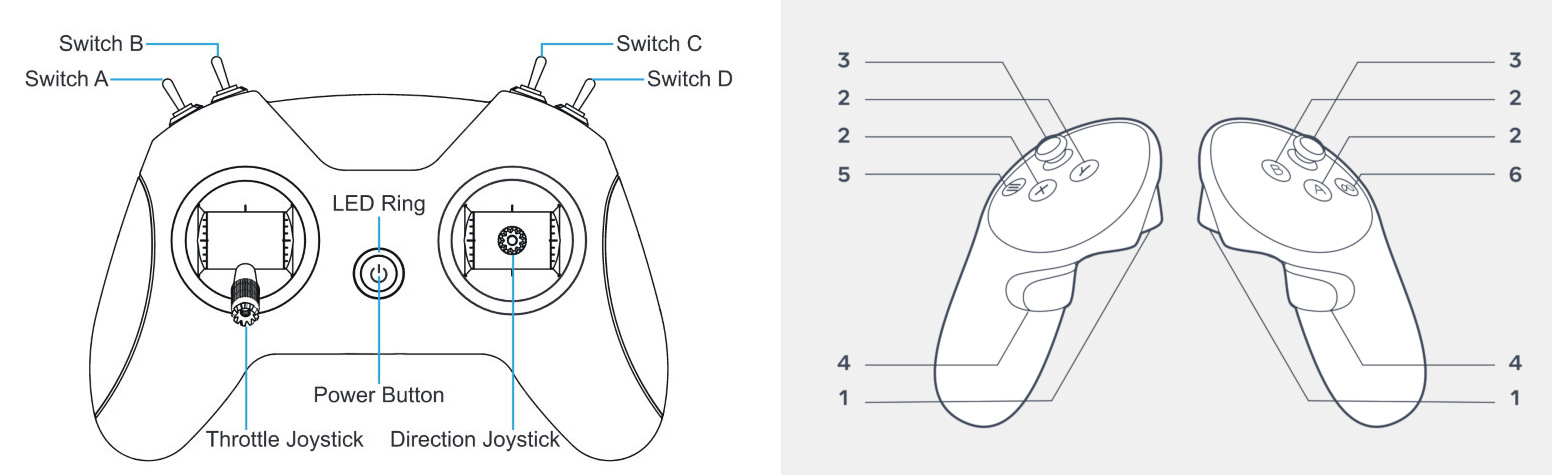
\includegraphics[width=0.8\linewidth]{img/control.jpg}
    \begin{flushleft}
    \small Adapted from \parencite{betafpv2022manual}
    \end{flushleft}
\end{figure}

The industry standardizes these controls into two primary layouts: Mode 1 (Japanese Hand): Predominantly used in Japan and parts of Europe. The throttle is located on the right gimbal; Mode 2 (American Hand): The global standard for FPV. The throttle is located on the left gimbal, which most pilots find more intuitive for separating altitude from directional pitch. Difference between Mode 1 and Mode 2 is shown in \cref{table:modes}

\begin{table}[h]
\caption{Comparison of Transmitter Control Modes}\label{table:modes}
\centering
\begin{tabular}{lllll}
\toprule
Mode & Left Stick (V) & Left Stick (H) & Right Stick (V) & Right Stick (H) \\
\midrule
Mode 1 & Pitch          & Yaw            & Throttle         & Roll            \\
Mode 2 & Throttle       & Yaw            & Pitch            & Roll            \\
\bottomrule
\end{tabular}
\end{table}

From a signal processing perspective, the flight controller differentiates between the unipolar throttle and the bipolar command sticks: Throttle ($T$): Mapped to a range of $[0, 1]$. Roll, Pitch, and Yaw ($\phi, \theta, \psi$): Mapped to a range of $[-1, 1]$. In \cref{fig:mode2} shows the interaction of the transmitter in Mode 2 and how the quadcopter move.

\begin{figure}
    \caption{Mode 2 control system}\label{fig:mode2}
    \centering
    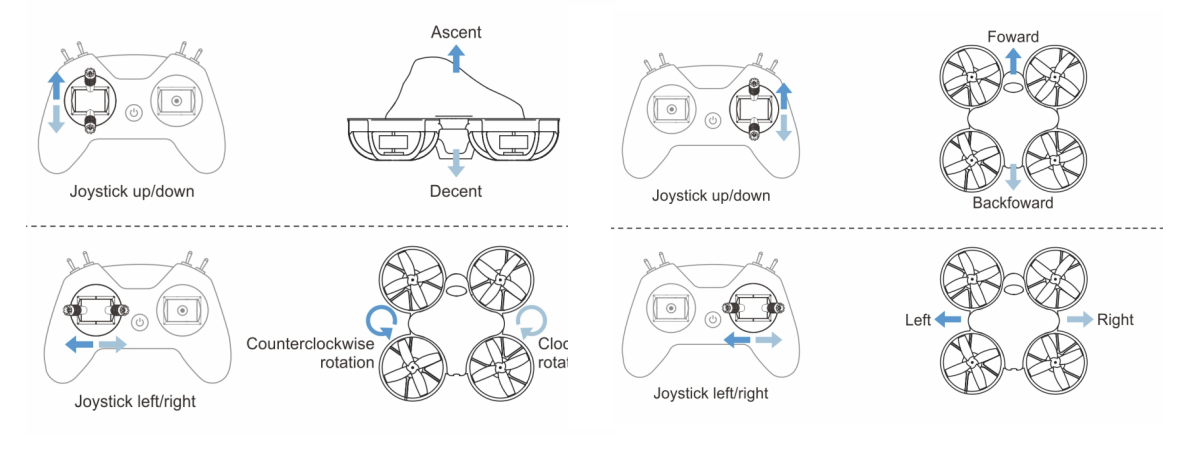
\includegraphics[width=0.8\linewidth]{img/drone.png}
    \begin{flushleft}
        \small Adapted from \parencite{betafpv2022manual}
    \end{flushleft}
\end{figure}


FPV drones generally operate across two flight logic modes. Self-Leveling (Angle/Normal Mode): The onboard flight controller uses accelerometers to automatically return the drone to a level horizon when the sticks are centered. This is ideal for beginners but limits maneuverability; Acrobat (Manual Mode): The controller only uses gyroscopes to maintain the current angular rate. If the pilot moves the stick and returns it to center, the drone maintains its current tilted orientation. This allows for flips and rolls but requires constant manual correction.

The FPV goggles provide the pilot with a low-latency first person view video feed pass from the camera set on the quadcopter's front. Beyond the video feed, an On-Screen Display (OSD) provides critical telemetry data, including battery voltage, signal strength, and flight time, as shown in \cref{fig:goggles}.

\begin{figure}
    \caption{The FPV goggles interface}\label{fig:goggles}
    \centering
    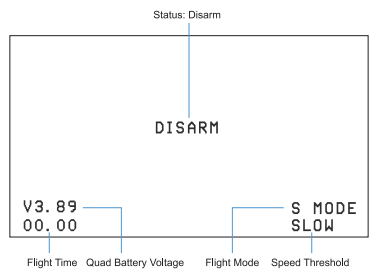
\includegraphics[width=0.8\linewidth]{img/goggles.png}
    \begin{flushleft}
        \small Adapted from \parencite{betafpv2022manual}
    \end{flushleft}
\end{figure}

\subsubsection{Proportional Integral and Derivative (PID) Control}\label{sec:pid}

In 1922, Nicolas Minorsky presented a very clear analysis of the control actions necessary to provide effective control of a system whose exact dynamics were un- known. He analyzed the actions taken by a good helmsman steering a ship and translated these actions into the appropriate mathematical formulations \parencite{bennett1993pid}. It is now know as the Proportional-Integral-Derivative (PID) controller. PID is a type of controller that is most commonly used and applied in mechanical systems \parencite{idrissi_review_2022}. Also used in many modern quadcopters, PID is employed here to stabilize drone movement and to function as a trainer AI.

The controller consists of three main components: Proportional ($K_p$): Acts like a virtual spring that pulls the system toward the desired position; the control action increases as the error gets larger; Integral ($K_i$): Accumulates the error over time to eliminate steady-state error, ensuring the drone reaches the exact target even in the presence of disturbances like gravity; Derivative ($K_d$): Acts as a virtual damper to reduce oscillations and prevent the system from overshooting its target.

The idealized control law is expressed as \cref{eq:pid}.

\begin{equation}\label{eq:pid}
    u(t) = K_p e(t) + K_i \int e(t) dt + K_d \frac{de(t)}{dt}
\end{equation}

PID control should be applied with careful parameter tuning, as the integral term ($K_i$) may introduce undesirable effects. While the integral component is essential for eliminating steady-state error,  improperly tuned integral action can lead to increased overshoot behavior. This phenomenon is commonly associated with integral windup and delayed error correction, as illustrated in \cref{fig:pd}.

\begin{figure}[H]
    \caption{Comparison of PID and PD}\label{fig:pd}
    \centering
    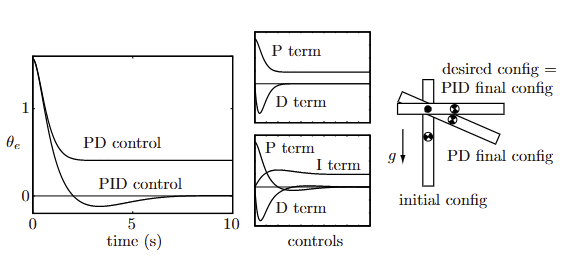
\includegraphics[width=0.8\linewidth]{img/pid.png}
    \begin{flushleft}
    \textit{Note. Adapted from \parencite{lynch2017modern}} 
    \end{flushleft}
\end{figure}

In certain applications, such as real-time drone attitude stabilization, a Proportional-Derivative (PD) controller may be sufficient. This is because the primary objective in such scenarios is to achieve fast and stable responses rather than eliminating steady-state error entirely. Moreover, user-controlled inputs, such as joystick commands, do not necessarily require exact convergence to a fixed reference value. As a result, omitting the integral component can simplify the control system and improve responsiveness.



